% chktex-file 44 32 36 38 18 11 8 26

\pagestyle{DS_FP}
%\NomPrenomNote{}

\bigskip


\section*{PARTIE A~--~Etude de la charge d'un condensateur}

On considère un circuit électrique dans lequel un condensateur se charge à partir d'une source de tension continue. On étudie dans cette partie la charge de ce condensateur.

\begin{minipage}{8cm}

\includegraphics[scale=0.45]{image2_6.jpg}

\end{minipage}
\begin{minipage}{10cm}
La loi des mailles en électricité nous donne:$E=Ri(t)+u(t)$
L'intensité circulant à l'intérieur d'un condensateur s'exprimant par $i=C\, \dfrac{du}{dt}$, on peut écrire:
\[\boxed{E=RC\, \dfrac{du(t)}{dt}+u(t)=RC\, u'(t)+u(t)}\]
\end{minipage}

En prenant $R=1\, k\Omega$, $C=100 \, \mu F$ et $E=5\, V$, on obtient l'équation différentielle suivante:

\[\boxed{(E):\, u'(t)+10\, u(t)=50}\]

\begin{enumerate}[series=monDS, resume]
    \item Vérifier que $u_p(t)=5$ est une solution particulière de cette équation différentielle.
    
    \begin{blocvisiblex}[height=2]
    {\quad}
    $u_p'(t)=0$ et $10\, u_p(t)=10 \times 5=50$, ainsi $u_p'(t)+10\, u_p(t)=50$.
    
        Donc $u_p(t)=5$ est une solution particulière de l'équation différentielle $(E)$.
\end{blocvisiblex}
    
    \medskip

    \item On considère l'équation différentielle homogène associée à l'équation différentielle précédente, c'est à dire l'équation différentielle suivante: \fbox{$(E_0):\, u'(t)+10\, u(t)=0$}. \par
    Justifier que la fonction $u_h$ définie par \fbox{$u_h(t)=A \e^{-10t}$} est une solution de cette équation différentielle homogène. ($A$ est une constante réelle à déterminer.)
    
    \begin{blocvisiblex}[height=3]
    {\quad}
    $u_h'(t)=-10A \e^{-10t}$ et $10\, u_h(t)=10A \e^{-10t}$, ainsi $u_h'(t)+10\, u_h(t)=0$.
    
        Donc la fonction $u_h$ définie par $u_h(t)=A \e^{-10t}$ est une solution de l'équation différentielle homogène $(E_0)$.
    \end{blocvisiblex}

    \medskip

    \item A $t=0$, le condensateur est déchargé, c'est à dire que \fbox{$u(0)=0$}. Exprimer la solution générale de l'équation différentielle $(E)$ en fonction de $A$ puis déterminer la valeur de $A$ vérifiant cette condition initiale.
    
    \begin{blocvisiblex}[height=2]
    {\quad}

    La solution générale de l'équation différentielle $(E)$ est de la forme $u(t)=u_p(t)+u_h(t)$. Ainsi $u(t)=5 + A \e^{-10t}$.

    En utilisant la condition initiale $u(0)=0$, on obtient $0=5 + A \e^{-10 \times 0}$ soit $A=-5$.
\end{blocvisiblex}
    \end{enumerate}

    \medskip

    On suppose maintenant que la fonction $f$ définie par \fbox{$f(t)=5\cdot (1 - \e^{-10t})$} est la solution de l'équation différentielle $(E)$ vérifiant la condition initiale $u(0)=0$.

\begin{enumerate}[series=monDS, resume]

\item Le temps $t$ étant exprimé en millisecondes, déterminer par la méthode de votre choix à partir de quelle valeur de $t$ la tension $f(t)$ devient supérieure à 4 volt. (On donnera une valeur approchée à $10^{-2}$ près.)
\begin{blocvisiblex}[height=3]
    {\quad}
    $f(t)>4 \Leftrightarrow 5\cdot (1 - \e^{-10t})>4 \Leftrightarrow 1 - \e^{-10t}>\dfrac{4}{5} \Leftrightarrow \e^{-10t}<\dfrac{1}{5}$ 

    $\Leftrightarrow -10t<\ln\left(\dfrac{1}{5}\right) \Leftrightarrow t>\dfrac{\ln(5)}{10}\approx 0,16$ ms.
    \end{blocvisiblex}

    \medskip    


%\item Montrer que la fonction $F$ définie par $F(t)= -\frac{5}{2} \e^{-2t}$ est une primitive de $f$ sur $\fo{0}{+\infty}$.
%\begin{blocvisiblex}[height=3]
%    {\quad}
%    \end{blocvisiblex}
%    \medskip


%    \item Déterminer la tension moyenne $\mu$ aux bornes du condensateur pendant les 5 premières millisecondes.
%    \begin{blocvisiblex}[height=3]
%    {\quad}
%    \end{blocvisiblex}    
   \end{enumerate}


%    \bigskip
    \pagebreak

    \section*{PARTIE B~--~Etude probabiliste}

\bigskip

\begin{minipage}{0.48\textwidth}
Ces condensateurs sont fabriqués par 2 usines différentes, l'usine A et l'usine B. L'usine A produit 60\% des condensateurs et génère 3\% de défectueux, tandis que l'usine B produit 40\% des condensateurs et génère 7\% de défectueux.

Un condensateur est prélevé au hasard en sortie de chaîne.

On note les évènements suivants:

\begin{itemize}
    \item $D$: « le condensateur est défectueux »,
    \item $A$: « le condensateur provient de la ligne A » et
    \item $B$: « le condensateur provient de la ligne B ».
\end{itemize}


\medskip



\end{minipage}\hfill{}
\begin{minipage}{0.48\textwidth}
    \begin{blocvisiblex}[height=6]
    {\begin{center}
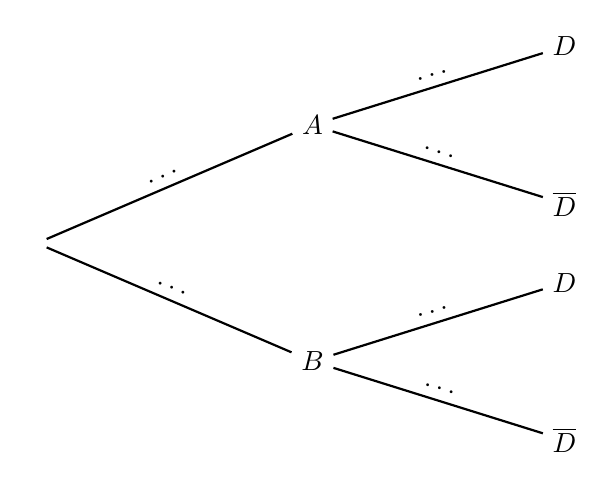
\begin{tikzpicture}[
    grow=right,     % On définit la croissance vers la droite
    % Réglages des distances entre les niveaux et les branches
    level 1/.style={sibling distance=3cm, level distance=3.5cm},
    level 2/.style={sibling distance=2cm, level distance=3.2cm},
    every node/.style={sloped}, % Aligne le texte sur les branches
    edge from parent/.style={draw, thick} % Ajoute une flèche au bout
]
% Racine
\node {} 
    child { node {$B$}
        child { node {$\overline{D}$} 
            edge from parent node[above] {$\ldots{}$} }
        child { node {$D$} 
            edge from parent node[above] {$\ldots{}$} }
        edge from parent node[above] {$\ldots{}$} }
    child { node {$A$}
        child { node {$\overline{D}$} 
            edge from parent node[above] {$\ldots{}$} }
        child { node {$D$} 
            edge from parent node[above] {$\ldots{}$} }
        edge from parent node[above] {$\ldots{}$} }
    ;
\end{tikzpicture}
\end{center}}
\begin{center}
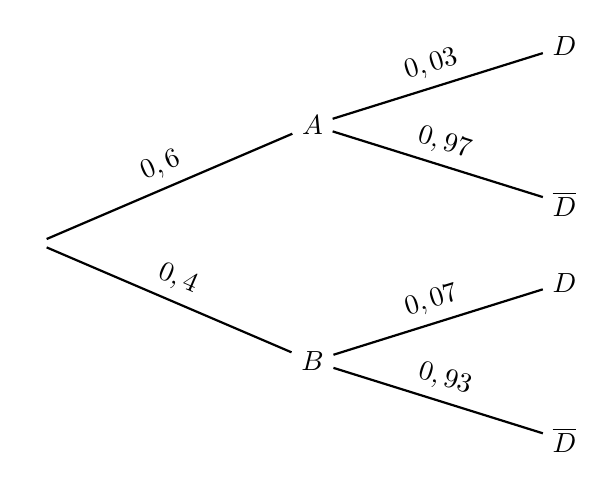
\begin{tikzpicture}[
    grow=right,     % On définit la croissance vers la droite
    % Réglages des distances entre les niveaux et les branches
    level 1/.style={sibling distance=3cm, level distance=3.5cm},
    level 2/.style={sibling distance=2cm, level distance=3.2cm},
    every node/.style={sloped}, % Aligne le texte sur les branches
    edge from parent/.style={draw, thick} % Ajoute une flèche au bout
    %edge from parent/.style={draw, -latex, thick} % Ajoute une flèche au bout
]
% Racine
\node {} 
    child { node {$B$}
        child { node {$\overline{D}$} 
            edge from parent node[above] {$0,93$} }
        child { node {$D$} 
            edge from parent node[above] {$0,07$} }
        edge from parent node[above] {$0,4$} }
    child { node {$A$}
        child { node {$\overline{D}$} 
            edge from parent node[above] {$0,97$} }
        child { node {$D$} 
            edge from parent node[above] {$0,03$} }
        edge from parent node[above] {$0,6$} }
    ;
\end{tikzpicture}
\end{center}
    \end{blocvisiblex}
\end{minipage}


\begin{enumerate}[series=monDS, resume]
    \item Compléter l'arbre de probabilité ci-contre.
    \medskip

    \item Calculer la probabilité que le condensateur prélevé soit défectueux et provienne de la ligne A.
    \begin{blocvisiblex}[height=2.]
    {\quad}
    $P(A\cap D)=P(A) \times P_D(A)=0,6 \times 0,03=0,018$
    \end{blocvisiblex}
    \medskip
    \item Montrer que la probabilité que le condensateur prélevé soit défectueux est égale à \fbox{$0,046$}.
    \begin{blocvisiblex}[height=2.]
    {\quad}
    $P(D)=P(A\cap D)+P(B\cap D)=P(A) \times P_D(A)+P(B) \times P_D(B)=0,6 \times 0,03+0,4 \times 0,07=0,046$
    \end{blocvisiblex}
    \medskip
    %\item Calculer $P_D(A)$ et donner une interprétation de cette valeur dans le contexte de l'exercice.
    %\begin{blocvisiblex}[height=2.5]
    %{\quad}
    %\end{blocvisiblex}
    %\medskip
\end{enumerate}


    %On prélève un échantillon de 30 condensateurs indépendamment les uns des autres. On admet que la probabilité qu'un condensateur soit défectueux est \fbox{$0,046$}

%Soit $X$ la variable aléatoire qui compte le nombre de condensateurs défectueux dans l'échantillon. On supposera que cette variable aléatoire suit une loi binomiale.

%\begin{enumerate}[series=monDS, resume]

    %\item Déterminer la probabilité qu'au moins 2 condensateurs soient défectueux dans l'échantillon.
    %\begin{blocvisiblex}[height=1.5]
    %{\quad}
    %\end{blocvisiblex}
%\end{enumerate}


%\pagebreak

La durée de vie du condensateur, exprimée en années est modélisée par une variable aléatoire $Y$ qui suit la loi exponentielle de paramètre \fbox{$\lambda=0,2$}.

On rappelle que la densité de probabilité de la loi exponentielle de paramètre $\lambda$ est donnée par la fonction $f$ définie par:
\[\boxed{f(t) = \lambda e^{-\lambda t}, \quad t \geq 0 \qquad \text{ et } \qquad P(X \geq a) = e^{-\lambda a}}\]

\begin{enumerate}[series=monDS, resume]
    \item A quel instant $t$, la probabilité qu'un condensateur tombe en panne pour la première fois est de \fbox{$0,5$}?
    \begin{blocvisiblex}[height=1.5]
    {\quad}
    $P(Y \geq t)=0,5 \Leftrightarrow e^{-0,2t}=0,5 \Leftrightarrow -0,2t=\ln(0,5) \Leftrightarrow t=\dfrac{\ln(2)}{0,2}\approx 3,47$ ans.
    \end{blocvisiblex}  
        \medskip
    \item Calculer la probabilité qu'un condensateur fonctionne toujours au bout de 2 ans.
    \begin{blocvisiblex}[height=1.5]
    {\quad}
    $P(Y \geq 2)=e^{-0,2 \times 2}=e^{-0,4}\approx 0,6703$.
    \end{blocvisiblex}  
        \par\medskip
    \item Calculer la probabilité qu'un condensateur fonctionne toujours au bout de 3 ans sachant qu'il fonctionne toujours au bout de 2 ans.
	\begin{blocvisiblex}[height=2]
    {\quad}
        $P(Y \geq 3|Y \geq 2)=P(Y \geq 1)=0,8187$.
\end{blocvisiblex} 

\end{enumerate}

\pagebreak

\thispagestyle{DS_LP}

\section*{PARTIE C~--~Discrétisation de l'étude du signal de charge d'un condensateur}

\bigskip

Dans la première partie, nous avons étudié la charge du condensateur en régime continu. Nous allons ici étudier la charge du condensateur en régime discrèt.


On rappelle que l'équation différentielle $(E)$ est définie par \fbox{$u'(t)+10\, u(t)=50$} et on suppose qu'à $t=0$, le condensateur est déchargé, c'est à dire que \fbox{$u(0)=0$}.

Pour étudier ce système numériquement, on choisit un pas de temps $h=0,01$ seconde. On définit la suite $(u_n)$ où $u_n$ représente une approximation de la tension $u(t)$ à l'instant $t_n=n \times h$.

On peut montrer qu'on peut remplacer $u'(t)$ par $\dfrac{u_{n+1}-u_n}{h}$ dans l'équation différentielle $(E)$.


\begin{enumerate}[series=monDS, resume]
    \item Montrer, en discrétisant l'équation différentielle $(E)$, que la suite $(u_n)$ vérifie la relation de récurrence suivante: \fbox{$u_{n+1}=0,9\, u_n + 0,5$} avec $u_0=0$.
    \begin{blocvisiblex}[height=4.5]
    {\quad}
    En remplaçant $u'(t)$ par $\dfrac{u_{n+1}-u_n}{h}$ dans l'équation différentielle $(E)$, on obtient:
\[\dfrac{u_{n+1}-u_n}{0,01}+10\, u_n=50\]
\[\Leftrightarrow u_{n+1}-u_n+0,1\, u_n=0,5\]
\[\Leftrightarrow u_{n+1}=0,9\, u_n + 0,5\]
    \end{blocvisiblex}
    \medskip

    \item A l'aide de la méthode de votre choix, déterminer à partir de quel rang $n$ la tension $u_n$ devient supérieure à 4 volts.
    \begin{blocvisiblex}[height=2.5]
    {\quad}
    En utilisant un tableur, on trouve que $u_{15}<4$ et $u_{16}>4$. Ainsi la tension $u_n$ devient supérieure à 4 volts à partir du rang $n=16$.
    \end{blocvisiblex}
    \par\par\medskip
    \medskip
    \item En déduire le temps en secondes à partir duquel la tension devient supérieure à 4 volts. Comparer ce résultat avec celui obtenu en question 1 de la partie A.
    \begin{blocvisiblex}[height=2.5]
    {\quad}
    La tension $u_n$ devient supérieure à 4 volts à partir du rang $n=16$, soit à partir du temps $t_{16}=16 \times 0,01=0,16$ secondes.

    \end{blocvisiblex}
    \par\par\medskip
    \item Montrer que la suite $(u_n)$ peut s'écrire sous la forme $u_n=5\cdot (1-0,9^n)$.
    \begin{blocvisiblex}[height=5]
    {\quad}
    On a $u_{n+1}=5\cdot (1-0,9^{n+1})$ et $u_n=5\cdot (1-0,9^n)$, ainsi:
\begin{align*}
    u_{n+1}&=5\cdot (1-0,9^{n+1})\\
    &=5\cdot (1-0,9^n)\cdot (1-0,9)\\
    &=5\cdot (1-0,9^n)\cdot 0,1\\
    &=5\cdot 0,9^n\\
    &=0,9 \cdot 5\cdot (1-0,9^n)+0,5
    &=0,9\, u_n + 0,5
\end{align*}

    \end{blocvisiblex}
    \medskip


    \end{enumerate}
\end{document}

\subsection*{Contexte général}

Une entreprise spécialisée dans les systèmes embarqués développe un nouveau module de transmission de données sans fil. Les équipes travaillent sur trois problématiques distinctes: la modélisation du signal de charge d'un condensateur, la gestion d'une mémoire tampon (buffer), et le contrôle qualité des modules produits.

\section*{PARTIE A~--~Contrôle de qualité}

\medskip

\emph{Dans cette partie, vous arrondirez toutes les valeurs à $10^{-4}$ si nécessaire.}

\medskip

 \begin{minipage}{0.48\textwidth}
L'usine produit des modules de transmission. Le service qualité distingue deux lignes de production:

\begin{itemize}
    \item la ligne A, qui produit $60\%$ des modules et génère $3\%$ de défectueux;
    \item la ligne B, qui produit $40\%$ des modules et génère $7\%$ de défectueux.
\end{itemize}

On note $D$ l'événement « le module est défectueux », $A$ l'événement « le module provient de la ligne A » et $B$ l'événement « le module provient de la ligne B ».

Un module est prélevé au hasard en sortie de chaîne.

\medskip

\begin{enumerate}[series=monDS, resume]
    \item Compléter l'arbre de probabilité ci-contre.
\end{enumerate}

\end{minipage}\hfill{}
\begin{minipage}{0.48\textwidth}
    \begin{blocvisiblex}[height=6]
    {\begin{center}
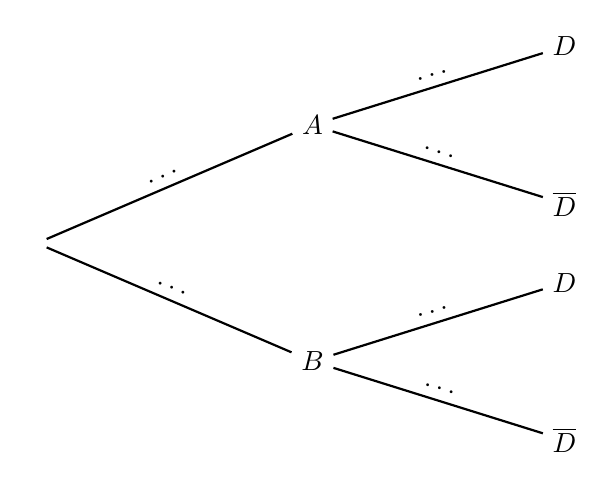
\begin{tikzpicture}[
    grow=right,     % On définit la croissance vers la droite
    % Réglages des distances entre les niveaux et les branches
    level 1/.style={sibling distance=3cm, level distance=3.5cm},
    level 2/.style={sibling distance=2cm, level distance=3.2cm},
    every node/.style={sloped}, % Aligne le texte sur les branches
    edge from parent/.style={draw, thick} % Ajoute une flèche au bout
]
% Racine
\node {} 
    child { node {$B$}
        child { node {$\overline{D}$} 
            edge from parent node[above] {$\ldots{}$} }
        child { node {$D$} 
            edge from parent node[above] {$\ldots{}$} }
        edge from parent node[above] {$\ldots{}$} }
    child { node {$A$}
        child { node {$\overline{D}$} 
            edge from parent node[above] {$\ldots{}$} }
        child { node {$D$} 
            edge from parent node[above] {$\ldots{}$} }
        edge from parent node[above] {$\ldots{}$} }
    ;
\end{tikzpicture}
\end{center}}
\begin{center}
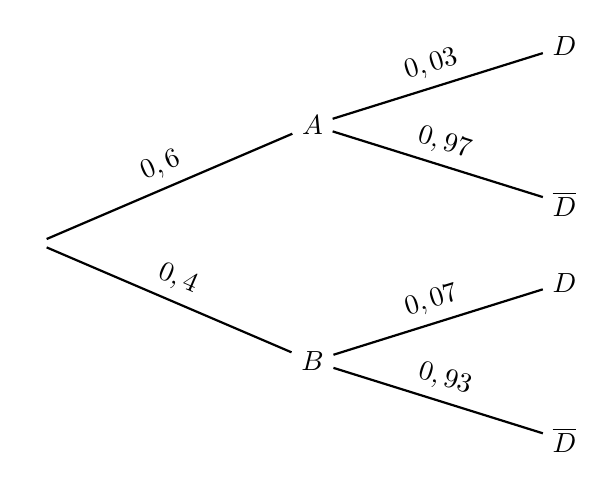
\begin{tikzpicture}[
    grow=right,     % On définit la croissance vers la droite
    % Réglages des distances entre les niveaux et les branches
    level 1/.style={sibling distance=3cm, level distance=3.5cm},
    level 2/.style={sibling distance=2cm, level distance=3.2cm},
    every node/.style={sloped}, % Aligne le texte sur les branches
    edge from parent/.style={draw, thick} % Ajoute une flèche au bout
    %edge from parent/.style={draw, -latex, thick} % Ajoute une flèche au bout
]
% Racine
\node {} 
    child { node {$B$}
        child { node {$\overline{D}$} 
            edge from parent node[above] {$0,93$} }
        child { node {$D$} 
            edge from parent node[above] {$0,07$} }
        edge from parent node[above] {$0,4$} }
    child { node {$A$}
        child { node {$\overline{D}$} 
            edge from parent node[above] {$0,97$} }
        child { node {$D$} 
            edge from parent node[above] {$0,03$} }
        edge from parent node[above] {$0,6$} }
    ;
\end{tikzpicture}
\end{center}
    \end{blocvisiblex}
\end{minipage}



    
\begin{enumerate}[resume=monDS]
    \item Calculer la probabilité que le module prélevé soit défectueux et provienne de la ligne A.
     \begin{blocvisiblex}[height=2.5]
    {\quad}
    $P(A\cap D)=P(A) \times P_D(A)=0,6 \times 0,03=0,018$

    \smallskip
    La probabilité que le module prélevé soit défectueux et provienne de la ligne A est de $0,018$.
     \end{blocvisiblex}
     \medskip
    \item Montrer que la probabilité que le module prélevé soit défectueux est égale à \fbox{$0,046$}.
    \begin{blocvisiblex}[height=2.5]
    {\quad}
    $P(D)=P(A\cap D)+P(B\cap D)=P(A) \times P_D(A)+P(B) \times P_D(B)=0,6 \times 0,03+0,4 \times 0,07=0,046$

        \smallskip
    La probabilité que le module prélevé soit défectueux est de $0,046$.
    \end{blocvisiblex}
    \medskip
    \item Calculer $P_D(A)$ et donner une interprétation de cette valeur dans le contexte de l'exercice.
    \begin{blocvisiblex}[height=2.5]
    {\quad}
    $P_D(A)=\dfrac{P(A\cap D)}{P(D)}=\dfrac{P(A) \times P_D(A)}{P(D)}=\dfrac{0,6 \times 0,03}{0,046}\approx 0,3913$

        \smallskip
    La probabilité que le module provienne de la ligne A sachant qu'il est défectueux est d'environ $0,3913$.
     \end{blocvisiblex}
     \medskip
     
\end{enumerate}

Un technicien prélève un échantillon de \fbox{30} modules indépendamment les uns des autres. On admet que la probabilité qu'un module soit défectueux est \fbox{$0,046$}

Soit $X$ la variable aléatoire qui compte le nombre de modules défectueux dans l'échantillon. On supposera que cette variable aléatoire suit une loi binomiale.

\begin{enumerate}[series=monDS, resume]

\begin{minipage}{0.47\textwidth}
        \item Donner les paramètres de cette loi binomiale
\end{minipage}\hfill{}
\begin{minipage}{0.47\textwidth}
    \begin{blocvisiblex}[height=1]
    {\quad}
    $n=30$ et $p=0,046$
    \end{blocvisiblex}
\end{minipage}


\begin{minipage}{0.47\textwidth}
    \bigskip
    \item Déterminer la probabilité qu'au moins 2 modules soient défectueux dans l'échantillon.
\end{minipage}\hfill{}
\begin{minipage}{0.47\textwidth}
    \begin{blocvisiblex}[height=1]
    {\quad}
    $P(X\geq 2)= 0.4043$
    \end{blocvisiblex}
\end{minipage}
\end{enumerate}

\pagebreak
Le technicien souhaite que la probabilité de détecter au moins un module défectueux sur $n$ prélèvements soit supérieure à \fbox{$0,9$}.

\begin{enumerate}[series=monDS, resume]
    \item Montrer que cette condition s'écrit \fbox{${0,954}^n \leq 0,1$}.
    \begin{blocvisiblex}[height=3]
    {\quad}
    $P(X\geq 1)=1-P(X=0)=1-{(1-p)}^n=1-{0,954}^n$

    La condition $P(X\geq 1)\geq0,99$ s'écrit alors $1-{(1-p)}^n\geq 0,9$ soit ${0,954}^n \leq 0,1$.
    \end{blocvisiblex}
    \medskip
    \begin{minipage}{0.50\textwidth}
    \item A l'aide de Géogébra, déterminer à partir de quel valeur de $n$ la condition est satisfaite.
\end{minipage}\hfill{}
\begin{minipage}{0.43\textwidth}
    \begin{blocvisiblex}[height=1]
    {$n=\dotfill$}
    $n= 49$
    \end{blocvisiblex}
\end{minipage}

    \appelprof{}
\end{enumerate}

\medskip

\section*{PARTIE B~--~Modélisation du signal de charge d'un condensateur}

Un ingénieur modélise la tension aux bornes d'un condensateur lors d'une phase de charge par une fonction de la forme:

\[\boxed{f(t)=(at+b)\cdot \e^{-kt}}\qquad \text{où $a$, $b$ et $k$ sont des constantes réelles.}\]

\begin{itemize}
    \item $t$ est le temps en millisecondes (ms) depuis le début de la charge du condensateur.
    \item $f(t)$ est la tension en volts (V) aux bornes du condensateur à l'instant $t$.
    \item $k$ est un coefficient de décroissance qui modélise la résistance du circuit, influençant la rapidité avec laquelle la tension atteint son maximum et commence à décroître.
\end{itemize}

\subsection*{Etude d'un cas particulier}

    Dans cette partie uniquement, on considèrera que les constantes $a$, $b$ et $k$ prennent les valeurs suivantes:

    \begin{minipage}{0.28\textwidth}
\begin{itemize}
    \item $a=0$,
    \item $b=5$,
    \item $k=0,5$.
\end{itemize}
\end{minipage}\hfill{}
\begin{minipage}{0.68\textwidth}
    Ainsi la fonction $f$ s'exprime par: \fbox{$f(t)=5\cdot \e^{-0,5t}$}.

\end{minipage}



\begin{enumerate}[series=monDS, resume]
    \item Déterminer par le calcul une expression de la fonction dérivée $f'$ et montrer que \fbox{$f'(t)=-\dfrac{5}{2}\cdot \e^{-0,5t}$}.
    \begin{blocvisiblex}[height=2.8]
    {\quad}
    $f(t)= 5 \cdot \e^{-0,5t}$

    $f'(t)= 5 \cdot \Big(-0,5\cdot \e^{-0,5t}\Big)=-\dfrac{5}{2}\cdot \e^{-0,5t}$.
    \end{blocvisiblex}
    \medskip
    \item En déduire les variations de $f$ sur $\fo{0}{+\infty}$.
    \begin{blocvisiblex}[height=3]
    {\quad}
    $f'(t)$ est strictement négatif sur $\fo{0}{+\infty}$, ainsi $f$ est strictement décroissante sur $\fo{0}{+\infty}$.
    \end{blocvisiblex}

\end{enumerate}


\subsection*{Modélisation}

Dans cette partie, on considère que $a$, $b$ et $k$ sont des constantes réelles strictement positives, mais on ne connaît pas leurs valeurs.

Des études expérimentales ont permis de déterminer que:
\begin{itemize}
    \item la tension initiale $f(0)$ est de $5$ volts;
    \item la tension atteint un maximum au bout de $1,5$ ms.
    \item le coefficient de décroissance $k$ est égal à $0,5$.
\end{itemize}

La fonction $f$ est donc définie pour tout $t\geqslant 0$ par \fbox{$f(t)=(at+b)\cdot \e^{-0,5t}$}

\bigskip

\begin{enumerate}[series=monDS, resume]
    \begin{minipage}{0.48\textwidth}
    \item A l'aide des deux conditions expérimentales et à l'aide de Géogébra, déterminer les valeurs de $a$ et $b$.
\end{minipage}\hfill{}
\begin{minipage}{0.45\textwidth}
    \begin{blocvisiblex}[height=1.2]
    {$a=\dotfill \hspace{2cm} b=\dotfill$}
    $a=10 \hspace{2cm} b=5$
    \end{blocvisiblex}
\end{minipage}
    \appelprof{}
\end{enumerate}

\bigskip

Dans la suite de l'exercice on considèrera la fonction $f$ définie sur $\fo{0}{+\infty}$ par \fbox{$f(t)=5\cdot (2t+1)\cdot \e^{-0,5t}$}.

\begin{enumerate}[series=monDS, resume]
    \begin{minipage}{0.46\textwidth}
            \item Déterminer grâce à Géogébra l'expression factorisée de la fonction dérivée $f'$.

    \end{minipage}\hfill{}
    \begin{minipage}{0.48\textwidth}
\begin{blocvisiblex}[height=1.5]
    {\quad}

    \[f'(t)= \dfrac{5}{2}\cdot \Big(2t-3\Big)\cdot \e^{-0,5t}\]


    \end{blocvisiblex}
    \end{minipage}
    
    \medskip
    
    \item Déterminer par le calcul le signe de la fonction dérivée $f'(t)$ et compléter le tableau de variations de $f$ sur $\fo{0}{+\infty}$.
    \begin{blocvisiblex}[height=5.5]
    {
    \begin{minipage}{0.48\linewidth}
        \quad
    \end{minipage}\hfill{}
    \begin{minipage}{0.46\linewidth}
        \begin{tikzpicture}
                \tkzTabInit[lgt=1.8,espcl=2.3]
                {$t$ / 1, signe $\, f'(t)$ / 1, var \, $f$ / 2}
                {$0$,$\quad$, $+\infty$}
                \tkzTabLine{}
                \tkzTabVar{}
            \end{tikzpicture}
    \end{minipage}
    }
        \begin{minipage}{0.48\linewidth}
        $\e^{-0,5t}$ est strictement positif sur l'ensemble de définition. Ainsi le signe de $f'(t)$ est celui de $-\dfrac{5}{2}\big(2t-3\big)$.

        $2t-3$ est négatif sur $\fo{0}{1,5}$, nul en $t=1,5$ et positif sur $\fo{1,5}{+\infty}$.
    
        $f$ est donc croissante sur $\fo{0}{1,5}$, décroissante sur $\fo{1,5}{+\infty}$ et atteint un minimum en $t=1,5$.
    \end{minipage}\hfill{}
    \begin{minipage}{0.46\linewidth}
\begin{tikzpicture}
                \tkzTabInit[lgt=1.8,espcl=2.3]
                {$t$ / 1, signe $\, f'(t)$ / 1, var \, $f$ / 2}
                {$0$, ${1,5}$, $+\infty$}
                \tkzTabLine{,+,z,-,}
                \tkzTabVar{-/ $5$, +/ ${f(1,5)}$, -/ $0$}
            \end{tikzpicture}
        \end{minipage}
\end{blocvisiblex}
\end{enumerate}

\medskip


\begin{enumerate}[series=monDS, resume]
     
   \item Déterminer grâce à Géogébra à partir de quelle valeur de $t$ la tension $f(t)$ devient inférieure à 1 volt. (On donnera une valeur approchée à $10^{-2}$ près.)
    \begin{blocvisiblex}[height=1]
    {\quad}
    $f(t)<1$ à partir de $t\approx 9,14$ ms.
    \end{blocvisiblex}
\end{enumerate}

L'énergie dissipée en \textbf{joules} entre l'instant $a$ et l'instant $b$ est égal à $E=\displaystyle \int_{a}^{b} f(t) \dt$.

\begin{enumerate}[series=monDS, resume]
    \begin{minipage}{0.46\textwidth}
            \item Déterminer une primitive $F$ de $f$ sur $\fo{0}{+\infty}$.
    \end{minipage}\hfill{}
    \begin{minipage}{0.46\textwidth}
        \begin{blocvisiblex}[height=1.2]
    {\quad}

    \[F(t)=-10\cdot (2t+5)\cdot \e^{-0,5t}\]
    \end{blocvisiblex}
    \end{minipage}
    
    \medskip

    \item La fonction $F$ étant une primitive de $f$, quelle expression permet de calculer l'énergie $E$ dissipée entre l'instant $a$ et l'instant $b$? Cocher la bonne réponse:
   \begin{blocvisiblex}[height=1]
    {
    \faSquare[regular] \, $F(a) - F(b)$ \hfill \faSquare[regular] \, $F(b) - F(a)$ \hfill \faSquare[regular] \, $F(b)$ \hfill \faSquare[regular] \, $F(a)$ \hspace{1cm} 
 }         
    \faSquare[regular] \, $F(a) - F(b)$ \hfill \faCheck[regular] \, $F(b) - F(a)$ \hfill \faSquare[regular] \, $F(b)$ \hfill \faSquare[regular] \, $F(a)$ \hspace{1cm} 
    \end{blocvisiblex}
    \medskip
\item On suppose maintenant que l'énergie dissipée pendant les 5 premières milliseconde est égale à 40 joutes. Déterminer par le calcul l'énergie moyenne $\mu$ dissipée par milliseconde pendant les 5 premières millisecondes.
    \begin{blocvisiblex}[height=3]
    {\quad}
    L'énergie moyenne dissipée par milliseconde pendant les 5 premières millisecondes est $\mu=\dfrac{1}{5} \times 40=8$ joutes par milliseconde.
    \end{blocvisiblex}
    \medskip
    
\end{enumerate}
    

\bigskip

\thispagestyle{DS_LP}

%\thispagestyle{DS_LP}
\section*{PARTIE C~--~Gestion d'une mémoire tampon}

Un buffer (mémoire tampon) contient initialment 200 octets de données. A chaque cycle d'horloge, le système traite et supprime $10\%$ du contenu actuel du buffer.

On note $u_n$ la quantité de données (en octets) présente dans le buffer après $n$ cycles d'horloge.

\begin{enumerate}[series=monDS, resume]
    \item Justifier que la suite $(u_n)$ vérifie la relation de récurrence $u_{n+1}=0,9\cdot u_n$.
    \begin{blocvisiblex}[height=3.5]
    {\quad}
    La suite $(u_n)$ vérifie la relation de récurrence $u_{n+1}=0,9\cdot u_n$ car à chaque cycle d'horloge, le système traite et supprime $10\%$ du contenu actuel du buffer

    On a donc $u_{n+1}=u_n-0,1\cdot u_n=0,9\cdot u_n$.

    \end{blocvisiblex}
    \medskip
    \item Déterminer la nature de la suite $(u_n)$. 
    \begin{blocvisiblex}[height=2]
    {\quad}

    La suite $(u_n)$ est de la forme $u_{n+1}=q \times u_n$ avec $q=0,9$ constant, donc c'est une suite géométrique de raison $0,9$ et de premier terme $u_0=200$.
    \end{blocvisiblex}
    \medskip
    \item Exprimer $u_n$ en fonction de $n$. 
    \begin{blocvisiblex}[height=2]
    {\quad}
    $(u_n)$ est une suite géométrique de raison $0,9$ et de premier terme $u_0=200$, donc pour tout $n$ entier naturel, on a $u_n=u_0 \times q^n=200 \times 0,9^n$.
    \end{blocvisiblex}
    \medskip
    \begin{minipage}{0.45\textwidth}
    \item Compléter l'algorithme ci-dessous qui calcule le nombre de cycles d'horloges nécessaires pour que la quantité de données dans le buffer soit inférieure à 1 octet.

    \end{minipage}\hfill{}
    \begin{minipage}{0.46\textwidth}
    \begin{tcblisting}{%
  listing only,
  colback=white, 
  colupper=black, 
  title=Algorithme de recherche de seuil,
  boxsep=0pt,
  left=5mm,
  listing options={
    numbers=none,
    basicstyle=\ttfamily,
    escapeinside={(*}{*)},
    literate={<-}{{$\bm{\leftarrow}$}}2, % Ajout d'un petit espace après la flèche
    frame=none % Supprime le cadre interne de listings
    }
}
n <- 0
u <- 200
tant que (*\trou{u >= 1}*):
        u <- (*\trou{0,9 * u}*)
        n <- (*\trou{n + 1}*)
print(n)
\end{tcblisting}
    \end{minipage}
    \medskip

    \begin{minipage}{0.70\textwidth}
            \item Par la méthode de votre choix, déterminer le nombre de cycles d'horloge nécessaires pour que la quantité de données dans le buffer soit inférieure à 1 octet.
    \end{minipage}\hfill{}
    \begin{minipage}{0.20\textwidth}
\begin{blocvisiblex}[height=1.2]
{\quad}
  $n=51$
    \end{blocvisiblex}
    \end{minipage}
    
\end{enumerate}

\bigskip



